\documentclass{article}

\usepackage{graphicx}
\usepackage{tikz}
\usepackage{tikzsymbols}
\usetikzlibrary{calc,patterns,shapes.geometric}
\pagestyle{empty}
\usepackage[margin=0pt]{geometry}
\geometry{papersize={14in,12in}}

\def\centerarc[#1](#2)(#3:#4:#5){\draw[#1] ($(#2)+({#5*cos(#3)},{#5*sin(#3)})$) arc (#3:#4:#5);}

\begin{document}
	\begin{figure}
		\centering
		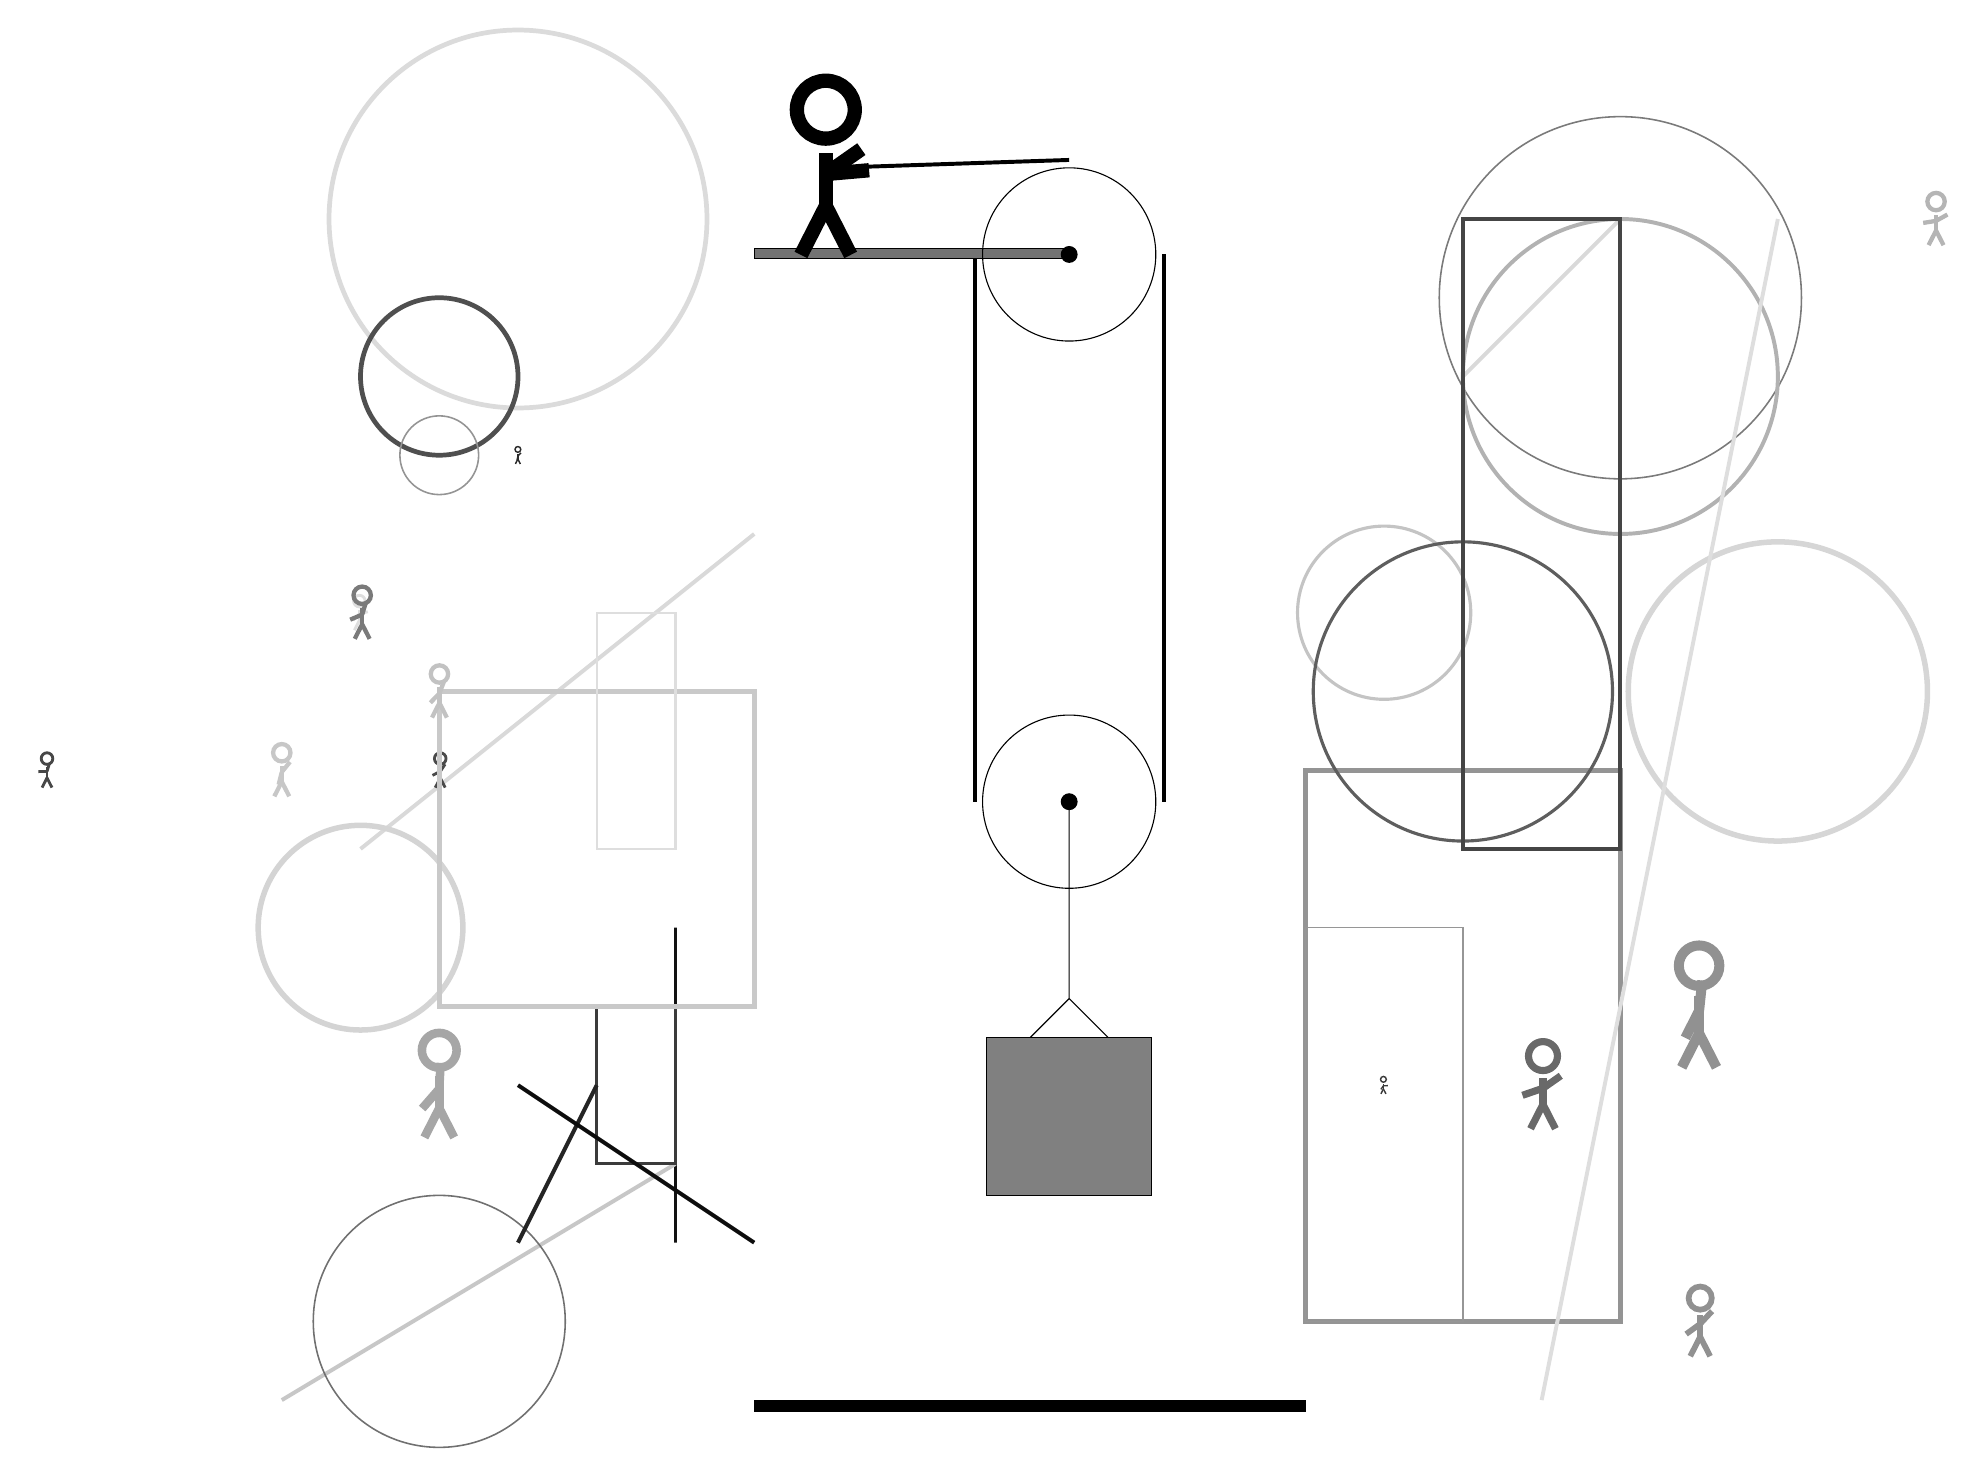
\begin{tikzpicture}
			%%%%% START %%%%%
			
			\draw[fill=black!55] (-2, 11.5) rectangle (2, 11.625);
			
			\draw (2, 4.6) circle (1.1);
			\draw[fill=black] (2, 4.6) circle (0.1);
			
			\draw (2, 11.55) circle (1.1);
			\draw[fill=black] (2, 11.55) circle (0.1);
			
			\draw (2, 4.6) -- (2, 2.1) -- (1.5, 1.6) -- (2.5, 1.6) -- (2, 2.1);
			\draw[fill=black!50] (0.95, 1.6) rectangle (3.05, -0.4);
			
			\node[line width=0.3mm, color=black!13] at (-7, 7) {\Strichmaxerl[2][45][15]};
			
			\draw[line width=0.5mm, color=black!15](-2, 8) -- (-7, 4);
			\draw[line width=0.7mm, color=black!14] (-4, 3) rectangle (-4, 3);
			\draw[line width=0.4mm, color=black!93] (-3, 3) rectangle (-3, -1);
			\node[line width=0.7mm, color=black!35] at (-6, 1) {\Strichmaxerl[6][49][87]};
			
			\node[line width=0.3mm, color=black!71] at (-6, 5) {\Strichmaxerl[2][27][56]};
			\node[line width=0.4mm, color=black!59] at (8, 1) {\Strichmaxerl[5][19][35]};
			\draw [line width=0.7mm, color=black!17](-7, 3) circle (1.3);
			\draw[line width=0.5mm, color=black!22](-3, 0) -- (-8, -3);
			\draw [line width=0.6mm, color=black!14](-5, 12) circle (2.4);
			\node[line width=0.5mm, color=black!83] at (-5, 9) {\Strichmaxerl[1][80][44]};
			
			\draw[line width=0.6mm, color=black!42] (5, 5) rectangle (9, -2);
			\draw [line width=0.4mm, color=black!23](6, 7) circle (1.1);
			
			\draw[line width=0.4mm, color=black!77] (-3, 0) rectangle (-4, 2);
			\draw [line width=0.6mm, color=black!69](-6, 10) circle (1.0);
			\draw [line width=0.2mm, color=black!52](9, 11) circle (2.3);
			
			\node[line width=0.6mm, color=black!29] at (13, 12) {\Strichmaxerl[3][9][29]};
			\draw[line width=0.2mm, color=black!17] (-2, 2) rectangle (-2, 3);
			\draw[line width=0.5mm, color=black!15](9, 12) -- (7, 10);
			\draw [line width=0.5mm, color=black!30](9, 10) circle (2.0);
			\draw [line width=0.2mm, color=black!42](-6, 9) circle (0.5);
			
			\draw [line width=0.2mm, color=black!56](-6, -2) circle (1.6);
			\draw [line width=0.4mm, color=black!63](7, 6) circle (1.9);
			\draw [line width=0.7mm, color=black!16](11, 6) circle (1.9);
			\node[line width=0.7mm, color=black!43] at (10, 2) {\Strichmaxerl[7][63][84]};
			
			\node[line width=0.7mm, color=black!22] at (-8, 5) {\Strichmaxerl[3][76][51]};
			\draw[line width=0.5mm, color=black!13](8, -3) -- (11, 12);
			\draw[line width=0.5mm, color=black!73] (7, 4) rectangle (9, 12);
			
			\draw[line width=0.5mm, color=black!86](-4, 1) -- (-5, -1);
			\node[line width=0.7mm, color=black!77] at (6, 1) {\Strichmaxerl[1][55][1]};
			\node[line width=0.2mm, color=black!72] at (-11, 5) {\Strichmaxerl[2][1][73]};
			
			\draw[line width=0.2mm, color=black!41] (5, -2) rectangle (7, 3);
			\draw[line width=0.5mm, color=black!95](-2, -1) -- (-5, 1);
			\node[line width=0.6mm, color=black!43] at (10, -2) {\Strichmaxerl[4][36][47]};
			\draw[line width=0.6mm, color=black!21] (-2, 2) rectangle (-6, 6);
			\node[line width=0.5mm, color=black!52] at (-7, 7) {\Strichmaxerl[3][23][73]};
			\node[line width=0.5mm, color=black!24] at (-6, 6) {\Strichmaxerl[3][46][69]};
			
			\draw[line width=0.3mm, color=black!13] (-4, 7) rectangle (-3, 4);
			
			\draw[line width=0.5mm] (0.8, 11.5) -- (0.8, 4.6);
			\centerarc[line width=0.5mm](2, 4.6)(180:360:1.2000000000000002);
			\draw[line width=0.5mm](3.2, 4.6) -- (3.2, 11.55);
			\centerarc[line width=0.5mm](2, 11.55)(0:90:1.2000000000000002);
			\draw[line width=0.5mm](2, 12.75) -- (-1, 12.65);
			
			\node at (-1, 12.65) {\Strichmaxerl[10][-175][35]};
			
			\draw[fill=black] (-2, -3) rectangle (5, -3.15);
			
			%%%%% END %%%%%
		\end{tikzpicture}
	\end{figure}	
\end{document}